\documentclass[oneside, a4paper ,12pt]{book}
\usepackage[utf8]{inputenc}
\usepackage{graphicx}
\graphicspath{{./images/}}

\begin{document}
	
	\author{Mochammad Hilmi Rusydiansyah \\ 5024211008}
	\title{Laporan Game \\ \emph{Bruh, RUN...!!!} \\ 
\includegraphics[width=8 cm]{ce.png}}
	\date{Desember 2022}
	
	\frontmatter
	\maketitle
	\tableofcontents
	
	\mainmatter
	\chapter{Pendahuluan}
	\section{Latar Belakang}
	
	Di zaman yang serba digital ini, \textit{game} tentu merupakan sesuatu yang sering kita dengar atau lihat dalam kehidupan sehari-hari. \textit{Game} sendiri adalah suatu hal yang kita gunakan sebagai media hiburan. Lebih jauh lagi, saat ini \textit{game} sudah merambah ke berbagai bidang sehingga memungkinkan \textit{game} menjadi sarana pendidikan, iklan, promosi, dan lain sebagainya. Hal itu membuat industri \textit{game} menjadi sangat masif. Bahkan industri \textit{game} saat ini sudah menyamai industri film-film terkenal seperti hollywood, membuat industri game menjadi salah satu industri terbesar yang ada saat ini. Selain itu, dengan banyaknya pengaplikasian \textit{game} tersebut, membuat game memiliki banyak jenis dan genre, dari \textit{pixel game} hingga \textit{triple A game}.
	
	Terlepas dari itu, \textit{game} sendiri merupakan suatu hal yang cukup kompleks. Dalam \textit{game}, tentunya kita harus menggabungkan unsur seni dan teknologi yang ada. Dimana keduanya merupakan dua hal yang cukup jauh dan tidak saling berkaitan. Seni sendiri sudah merupakan hal yang unik dan kadang abstrak jika kita baru menerjuninya, lalu ditambah teknologi sendiri yang merupakan hal yang butuh ketekunan dalam mempelajarinya.
	
	Di perkuliahan Struktur Data dan Analisa Algoritma semester ini, mahasiswa-mahasiswa yang diajar oleh dosen Pak Eko Mulyanto di kelas A diberikan suatu \emph{final project} yang mengharuskan para mahasiswa untuk membuat suatu \textit{game}. Game tersebut harus merupakan hasil karya masing-masing mahasiswa sesuai kemampuan yang dimiliki. Dalam pembuatannya, mahasiswa harus menggunakan bahasa C/C++ dan menggunakan \textit{library} yang menunjang dalam pengolahan grafik yang ada. Dimana \textit{library} yang digunakan tersebut adalah graphics.h atau sfml.
	
	\section{Penjelasan Game}
	
	\textit{Bruh, RUN...!!!} bercerita tentang seseorang yang terjebak di suatu savana. Sialnya, savana tersebut berisi banyak sekali kawanan serigala lapar yang siap menghabisi makhluk apapun yang berada di dalamnya. Dari sini lah \textit{game Bruh, RUN...!!!} dimulai. Pemain \textit{game} ini akan berperan sebagai seorang yang berada pada kesialan tersebut.
	
	Secara mekanisme, \textit{Bruh, RUN...!!!} merupakan sebuah \textit{game} yang memiliki konsep \textit{top-down shooter}. Dalam \textit{game} ini, pemain harus berusaha bertahan hidup dari serangan serigala yang datang dari segala arah dengan cara tidak terkena gigitan kawanan serigala tersebut. Untuk itu, pemain dapat menggocek dan mengecoh pergerakan kawanan serigala. Tiap serigala yang mengejar pemain memiliki kecepatan yang berbeda-beda satu sama lainnya. Hal ini membuat \textit{gameplay} yang lebih susah dibanding jika tiap serigala memiliki kecepatan yang sama.
	
	Selanjutnya, untuk menunjang tujuan tersebut, pemain memiliki amunisi yang sewaktu-waktu dapat dilemparkan ke kawanan serigala. Amunisi tersebut berupa daging, sehingga apabila daging terkena tepat ke salah satu serigala, maka serigala tersebut akan memakan daging tersebut. Hal ini tentu mengakibatkan serigala berhenti mengejar pemain karena rasa lapar yang ada pada serigala sudah terpenuhi dengan daging yang dilemparkan oleh pemain.
	
	Untuk selanjutnya, pemain juga memiliki \textit{health bar}. Dimana apabila pemain terlalu sering terkena gigitan serigala, maka pemain akan mati seiring habisnya \textit{health bar} yang ada. Mekanisme nilai bar ini juga diaplikasikan pada serigala. Apabila pemain memiliki \textit{health bar}, maka serigala di sini memiliki yang namanya \textit{hungry bar}. \textit{Hungry bar} ini memiliki fungsi menentukan apakah serigala masih mengejar pemain atau sudah kenyang. Jika sudah kenyang, tandanya serigala sudah tidak lagi mengejar pemain.
	
	\chapter{Desain}
	\section{Desain Game dan Karakter}
	\begin{figure} [h]
		\centering
		
\includegraphics[width=10 cm]{main_menu.png}
		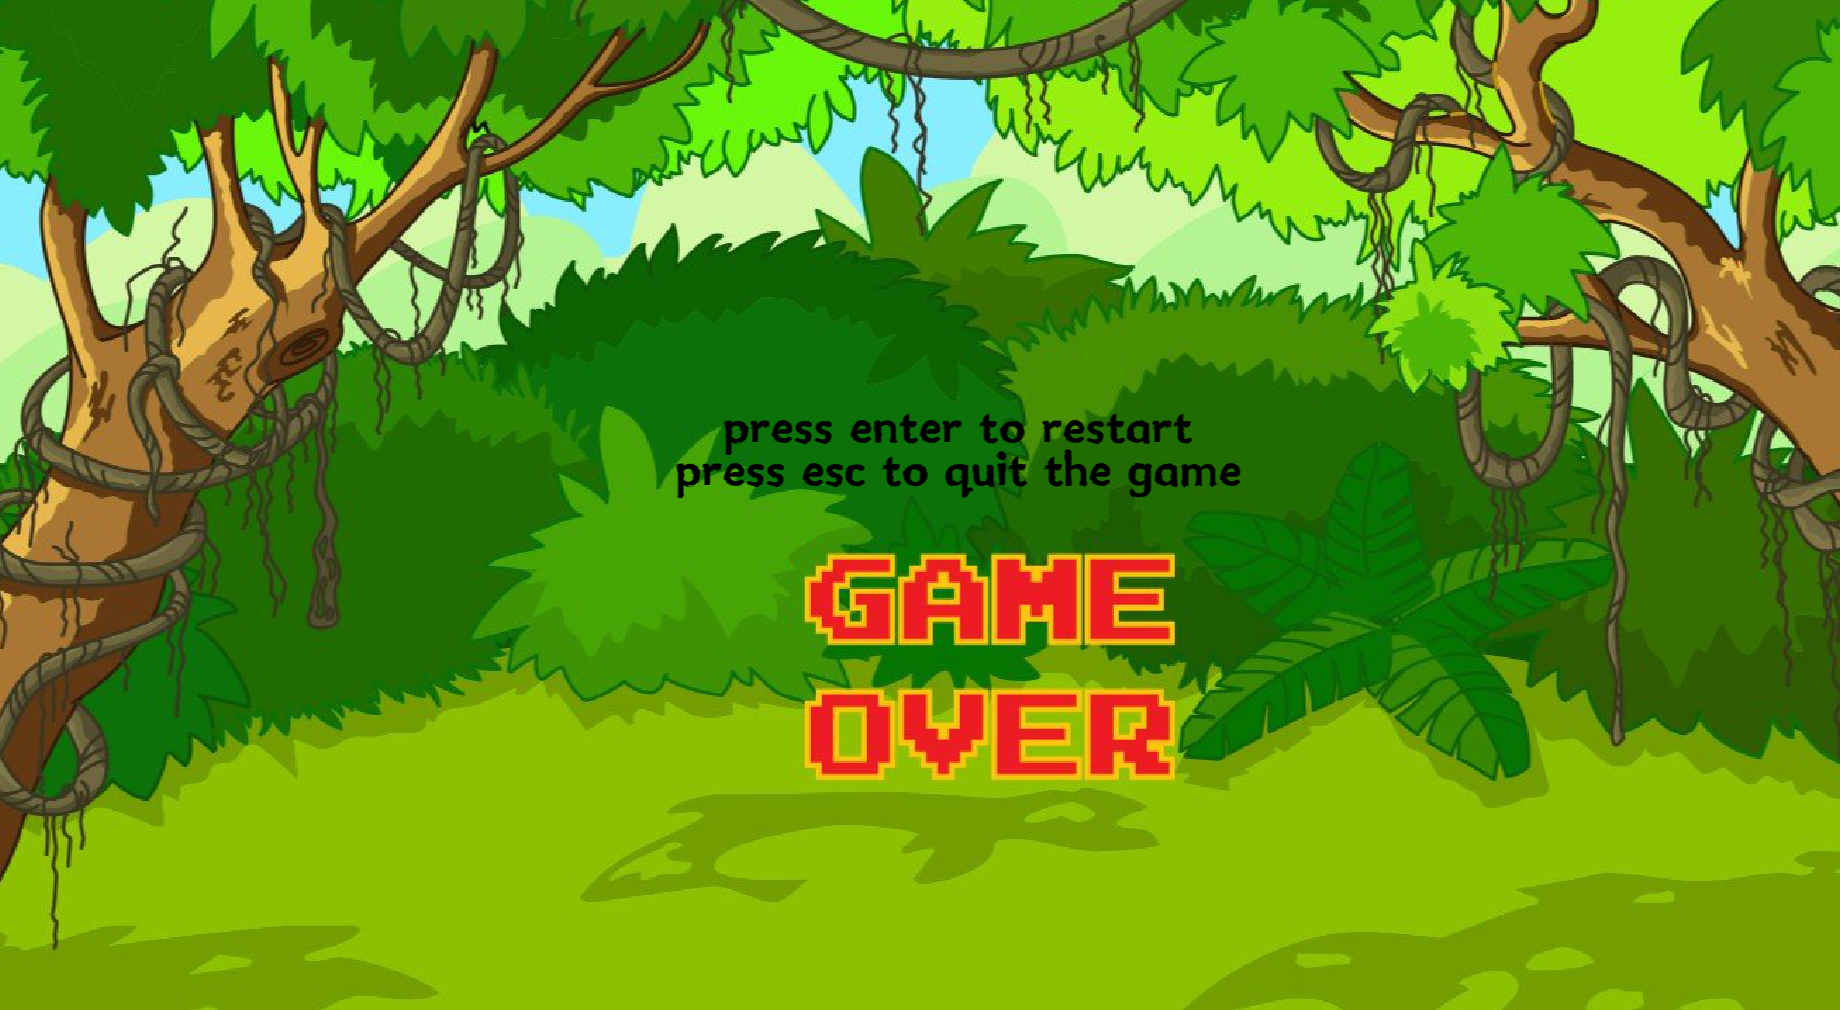
\includegraphics[width=10 cm]{game_over.png}
		\caption{Main Menu}
	\end{figure}
	\begin{figure} [h]
		\centering
		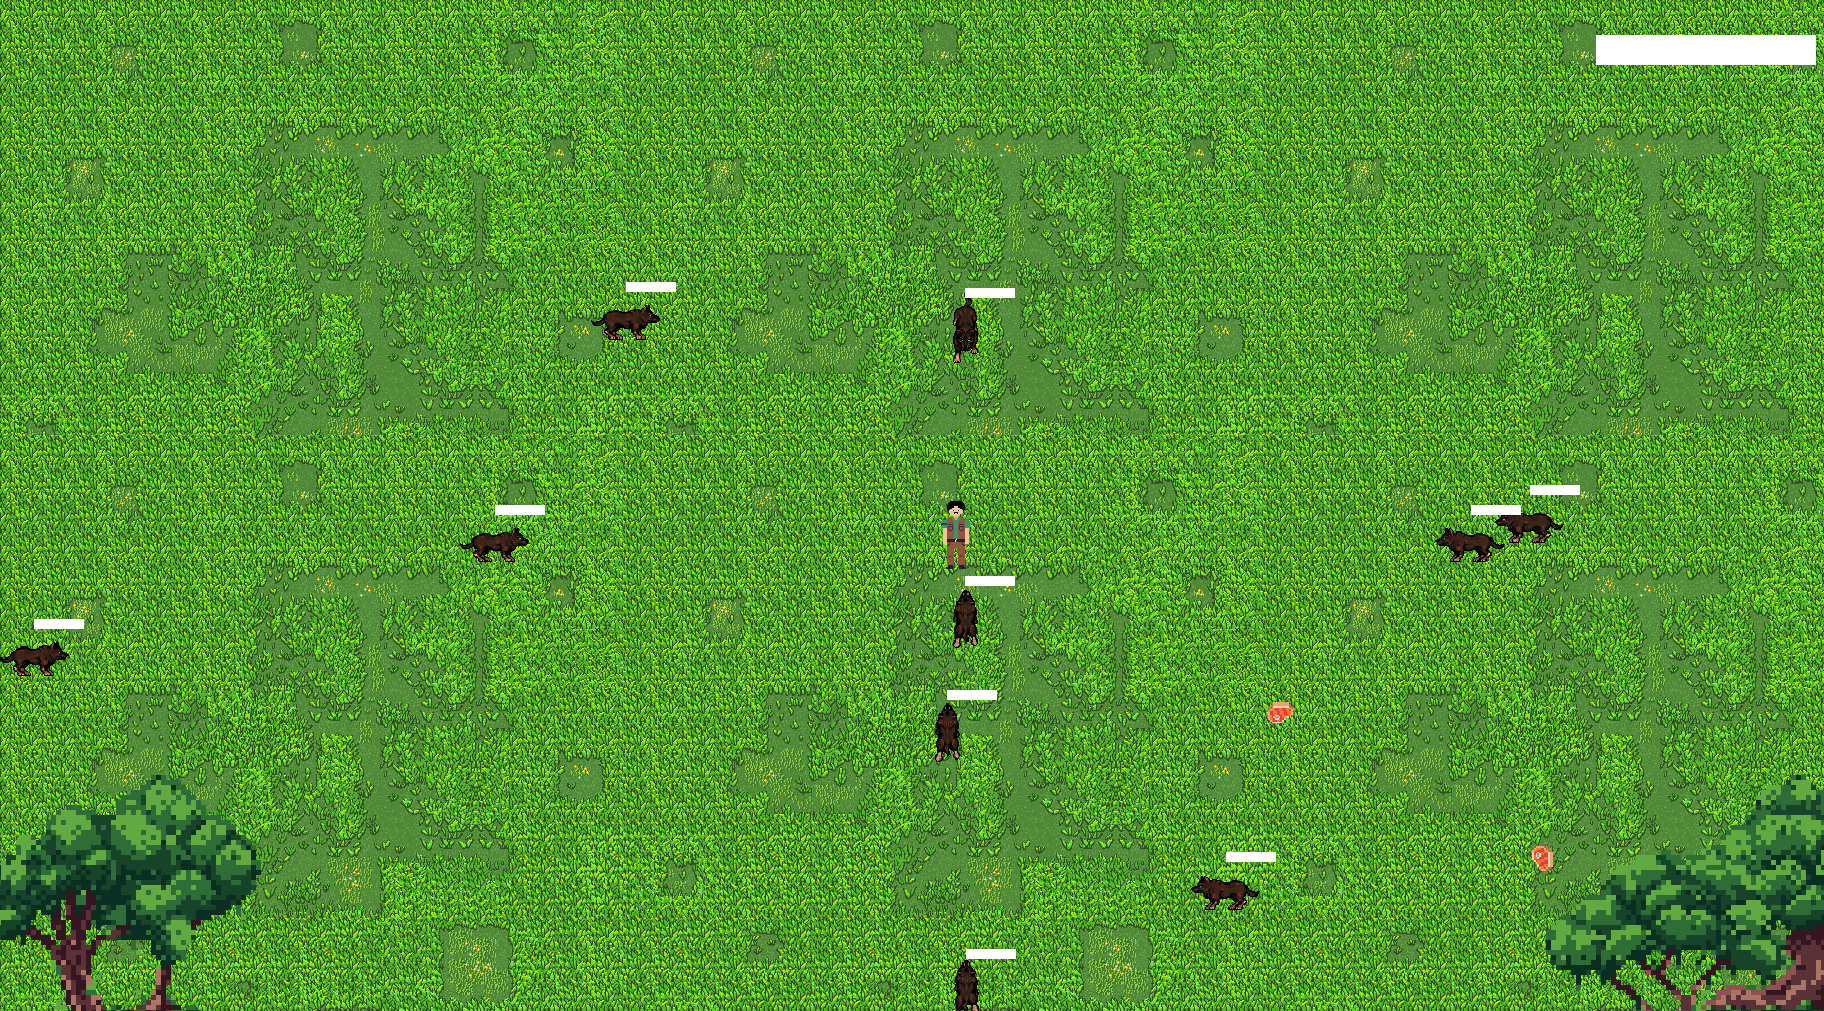
\includegraphics[width=10 cm]{in_game.png}
		\caption{Dalam Game}
	\end{figure}
	\begin{figure} [h]
		\centering
		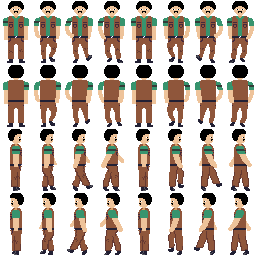
\includegraphics[width=10 cm]{lakon.png}
		\caption{Animasi Player}
	\end{figure}
	\begin{figure} [h]
		\centering
		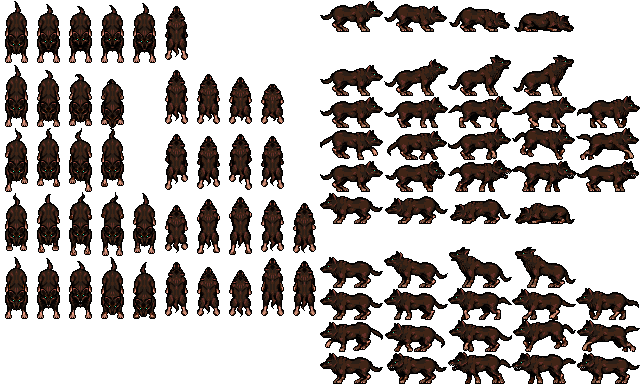
\includegraphics[width=10 cm]{wolf.png}
		\caption{Animasi Serigala}
	\end{figure}
	\begin{figure}
		\centering
		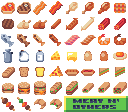
\includegraphics[width=10 cm]{MeatnOthers.png}
		\caption{Sprite Daging}
	\end{figure}
	\begin{figure} [h]
		\centering
		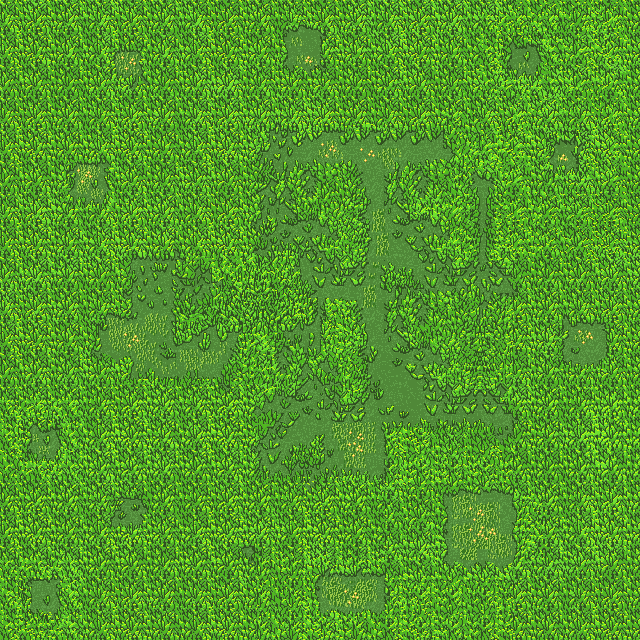
\includegraphics[width=10 cm]{grass.png}
		\caption{Sprite Rumput}
	\end{figure}
	\begin{figure}
		\centering
		
\includegraphics[width=10 cm]{48x48_trees.png}
		\caption{Sprite Pohon}
	\end{figure}
	
	
	\chapter{Struktur Data Karakter}
	
	\section{Codingan lakon.hpp}
	\begin{verbatim}
		#ifndef __LAKON_HPP__
		#define __LAKON_HPP__
		
		#include <SFML/Graphics.hpp>
		#include <SFML/System.hpp>
		#include <SFML/Window.hpp>
		#include <SFML/Audio.hpp>
		#include "global.hpp"
		#include <vector>
		
		class Lakon : public sf::Sprite{
			private:
			float health;
			int iter_anim;
			bool lakon_move;
			char command;
			char last_command;
			float speed;
			float clk_threshold;
			sf::Clock clk;
			sf::Vector2f vel;
			sf::Vector2i spriteSize;
			sf::Texture texture;
			std::vector<sf::IntRect> moveUpAnim;
			std::vector<sf::IntRect> moveLeftAnim;
			std::vector<sf::IntRect> moveDownAnim;
			std::vector<sf::IntRect> moveRightAnim;
			
			public:
			Lakon(float spd = 5){
				Lakon::health = 100.f;
				Lakon::clk_threshold = 0.05f;
				Lakon::iter_anim = 0;
				Lakon::lakon_move = false;
				Lakon::speed = spd;
				Lakon::vel = sf::Vector2f(0.f,0.f);
				Lakon::texture.loadFromFile("assets/images/lakon.png");
				Lakon::setTexture(texture);
				Lakon::spriteSize = sf::Vector2i(32, 64);
				Lakon::setTextureRect(sf::IntRect(0*spriteSize.x, 0*spriteSize.y, spriteSize.x, spriteSize.y));
				Lakon::setPosition(global::width_window/2, global::height_window/2);
				Lakon::setOrigin(spriteSize.x / 2, spriteSize.y / 2);
				Lakon::setScale(sf::Vector2f(1.1f, 1.1f));
				
				moveUpAnim.reserve(8);
				moveLeftAnim.reserve(8);
				moveDownAnim.reserve(8);
				moveRightAnim.reserve(8);
				for(int i=0; i<8; i++){
					moveDownAnim[i] = sf::IntRect(i*spriteSize.x, 0*spriteSize.y, spriteSize.x, spriteSize.y);
					moveUpAnim[i] = sf::IntRect(i*spriteSize.x, 1*spriteSize.y, spriteSize.x, spriteSize.y);
					moveRightAnim[i] = sf::IntRect(i*spriteSize.x, 2*spriteSize.y, spriteSize.x, spriteSize.y);
					moveLeftAnim[i] = sf::IntRect(i*spriteSize.x, 3*spriteSize.y, spriteSize.x, spriteSize.y);
				}
			}
			
			float get_health(){
				return Lakon::health;
			}
			
			void reduceHealth(float damage){
				if(Lakon::health <= 0){
					Lakon::health = 0;
				} else{
					Lakon::health = Lakon::health + damage;
				}
			}
			
			void displayHealth(sf::RenderWindow& window){
				sf::RectangleShape rectangle(sf::Vector2f((Lakon::health/100) * 220.f, 30.f));
				rectangle.setPosition(sf::Vector2f(1600.f, 40.f));
				
				window.draw(rectangle);
			}
			
			void movement(){
				Lakon::lakon_move = false;
				Lakon::command = '\0';
				if(sf::Keyboard::isKeyPressed(sf::Keyboard::W)){
					Lakon::vel.y = -1;
					Lakon::lakon_move = true;
					Lakon::command = 'w';
					Lakon::last_command = 'w';
				}
				else if(sf::Keyboard::isKeyPressed(sf::Keyboard::S)){
					Lakon::vel.y = 1;
					Lakon::lakon_move = true;
					Lakon::command = 's';
					Lakon::last_command = 's';
				}
				else Lakon::vel.y = 0;
				if(sf::Keyboard::isKeyPressed(sf::Keyboard::A)){
					Lakon::vel.x = -1;
					Lakon::lakon_move = true;
					Lakon::command = 'a';
					Lakon::last_command = 'a';
				}
				else if(sf::Keyboard::isKeyPressed(sf::Keyboard::D)){
					Lakon::vel.x = 1;
					Lakon::lakon_move = true;
					Lakon::command = 'd';
					Lakon::last_command = 'd';
				}
				else Lakon::vel.x = 0;
				
				if(Lakon::lakon_move){
					Lakon::vel = global::normalize(Lakon::vel);
					Lakon::vel.x = Lakon::vel.x * Lakon::speed;
					Lakon::vel.y = Lakon::vel.y * Lakon::speed;
					Lakon::move(Lakon::vel);
					Lakon::movement_animation();
				}else{  // if there is no command yet, set animation to "standing" mode
					switch(Lakon::last_command){
						case 'w':
						Lakon::setTextureRect(moveUpAnim[0]);
						break;
						case 's':
						Lakon::setTextureRect(moveDownAnim[0]);
						break;
						case 'a':
						Lakon::setTextureRect(moveLeftAnim[0]);
						break;
						case 'd':
						Lakon::setTextureRect(moveRightAnim[0]);
						break;
						default:
						Lakon::setTextureRect(moveDownAnim[0]);
					}
				}
			}
			
			void movement_animation(){
				if(clk.getElapsedTime().asSeconds() > Lakon::clk_threshold){
					if(Lakon::iter_anim == 7) iter_anim = -1;  // 0 to 7
					iter_anim++;
					// printf("%d\n", iter_anim);
					
					switch(Lakon::command){
						case 'w':
						Lakon::setTextureRect(moveUpAnim[iter_anim]);
						break;
						case 's':
						Lakon::setTextureRect(moveDownAnim[iter_anim]);
						break;
						case 'a':
						Lakon::setTextureRect(moveLeftAnim[iter_anim]);
						break;
						case 'd':
						Lakon::setTextureRect(moveRightAnim[iter_anim]);
						break;
					}
					clk.restart();
				}
			} 
		};
		
		#endif
	\end{verbatim}

	\section{Codingan animal.hpp}
	\begin{verbatim}
		#ifndef __ANIMAL_HPP__
		#define __ANIMAL_HPP__
		
		#include <SFML/Graphics.hpp>
		#include <SFML/System.hpp>
		#include <SFML/Window.hpp>
		#include <SFML/Audio.hpp>
		#include "global.hpp"
		#include <vector>
		
		class Animal : public sf::Sprite{
			private:
			float health;
			int iter_move_anim;
			int iter_bite_anim;
			bool lakon_move;
			char orientation;  // for determine wolf orientation, 'h' for horizontal, 'v' for vertical
			char command;
			char last_command;
			float speed;
			float clk_threshold;
			sf::Clock clk;
			sf::Vector2f vel;
			sf::Vector2i spriteSize_ver;
			sf::Texture texture;
			std::vector<sf::IntRect> moveUpAnim;
			std::vector<sf::IntRect> moveLeftAnim;
			std::vector<sf::IntRect> moveDownAnim;
			std::vector<sf::IntRect> moveRightAnim;
			std::vector<sf::IntRect> biteUpAnim;
			std::vector<sf::IntRect> biteDownAnim;
			std::vector<sf::IntRect> biteRightAnim;
			std::vector<sf::IntRect> biteLeftAnim;
			
			
			public:
			Animal(){
				Animal::health = 100.f;
				Animal::clk_threshold = 0.15f;
				Animal::iter_move_anim = 0;
				Animal::iter_bite_anim = 0;
				Animal::lakon_move = false;
				Animal::vel = sf::Vector2f(0.f,0.f);
				Animal::texture.loadFromFile("assets/images/wolf.png");
				Animal::setTexture(texture);
				Animal::orientation = 'v';
				Animal::spriteSize_ver = sf::Vector2i(32, 64);  // for vertical orientation
				Animal::setTextureRect(sf::IntRect(0*spriteSize_ver.x, 0*spriteSize_ver.y, spriteSize_ver.x, spriteSize_ver.y));
				Animal::setOrigin(spriteSize_ver.x / 2, spriteSize_ver.y / 2);  // for vertical orientation
				Animal::setScale(sf::Vector2f(1.1f, 1.1f));
				
				moveUpAnim.reserve(4);
				moveDownAnim.reserve(4);
				moveLeftAnim.reserve(5);
				moveRightAnim.reserve(5);
				for(int i=0; i<4; i++){
					moveDownAnim[i] = sf::IntRect(i*spriteSize_ver.x, 2*spriteSize_ver.y, spriteSize_ver.x, spriteSize_ver.y);
					moveUpAnim[i] = sf::IntRect((i+5)*spriteSize_ver.x, 2*spriteSize_ver.y, spriteSize_ver.x, spriteSize_ver.y);
				}
				for(int i=0; i<5; i++){
					moveRightAnim[i] = sf::IntRect((i+5)*spriteSize_ver.y, 3*spriteSize_ver.x, spriteSize_ver.y, spriteSize_ver.x);
					moveLeftAnim[i] = sf::IntRect((i+5)*spriteSize_ver.y, 9*spriteSize_ver.x, spriteSize_ver.y, spriteSize_ver.x);
				}
				biteUpAnim.reserve(5);
				biteDownAnim.reserve(5);
				biteRightAnim.reserve(5);
				biteLeftAnim.reserve(5);
				for(int i=0; i<5; i++){
					biteUpAnim[i] = sf::IntRect(i*spriteSize_ver.x, 4*spriteSize_ver.y, spriteSize_ver.x, spriteSize_ver.y);
					biteDownAnim[i] = sf::IntRect((i+5)*spriteSize_ver.x, 4*spriteSize_ver.y, spriteSize_ver.x, spriteSize_ver.y);
					biteRightAnim[i] = sf::IntRect((i+5)*spriteSize_ver.y, 5*spriteSize_ver.x, spriteSize_ver.y, spriteSize_ver.x);
					biteLeftAnim[i] = sf::IntRect((i+5)*spriteSize_ver.y, 11*spriteSize_ver.x, spriteSize_ver.y, spriteSize_ver.x);
				}
			}
			
			void set_speed(float inp_speed){
				Animal::speed = inp_speed;
			}
			
			float get_health(){
				return Animal::health;
			}
			
			void reduceHealth(float damage){
				if(Animal::health <= 0){
					Animal::health = 0;
				} else{
					Animal::health = Animal::health + damage;
				}
			}
			
			void displayHealth(sf::RenderWindow& window){
				sf::RectangleShape rectangle(sf::Vector2f((Animal::health/100) * 50.f, 10.f));
				rectangle.setPosition(sf::Vector2f(Animal::getPosition().x, Animal::getPosition().y - 40));
				
				window.draw(rectangle);
			}
			
			
			void movement(sf::Vector2f lakon_pos){
				Animal::lakon_move = false;
				Animal::command = '\0';
				if((lakon_pos.y - Animal::getPosition().y) < -10){
					Animal::vel.y = -1;
					Animal::lakon_move = true;
					Animal::command = 'w';
					Animal::last_command = 'w';
					Animal::orientation = 'v';
				}
				else if((lakon_pos.y - Animal::getPosition().y) > 10){
					Animal::vel.y = 1;
					Animal::lakon_move = true;
					Animal::command = 's';
					Animal::last_command = 's';
					Animal::orientation = 'v';
				}
				else Animal::vel.y = 0;
				if((lakon_pos.x - Animal::getPosition().x) < -10){
					Animal::vel.x = -1;
					Animal::lakon_move = true;
					Animal::command = 'a';
					Animal::last_command = 'a';
					Animal::orientation = 'h';
				}
				else if((lakon_pos.x - Animal::getPosition().x) > 10){
					Animal::vel.x = 1;
					Animal::lakon_move = true;
					Animal::command = 'd';
					Animal::last_command = 'd';
					Animal::orientation = 'h';
				}
				else Animal::vel.x = 0;
				
				if(Animal::lakon_move){
					Animal::vel = global::normalize(Animal::vel);
					Animal::vel.x = Animal::vel.x * Animal::speed;
					Animal::vel.y = Animal::vel.y * Animal::speed;
					Animal::move(Animal::vel);
					Animal::movement_animation();
				}else{
					Animal::bite_animation();
					
					//this is for quiet wolf animation
					// switch(Animal::last_command){
						//     case 'w':
						//         Animal::setTextureRect(moveUpAnim[3]);
						//         Animal::setOrigin(spriteSize_ver.x / 2, spriteSize_ver.y / 2);
						//         break;
						//     case 's':
						//         Animal::setTextureRect(moveDownAnim[3]);
						//         Animal::setOrigin(spriteSize_ver.x / 2, spriteSize_ver.y / 2);
						//         break;
						//     case 'a':
						//         Animal::setTextureRect(moveLeftAnim[0]);
						//         Animal::setOrigin(spriteSize_ver.y / 2, spriteSize_ver.x / 2);
						//         break;
						//     case 'd':
						//         Animal::setTextureRect(moveRightAnim[0]);
						//         Animal::setOrigin(spriteSize_ver.y / 2, spriteSize_ver.x / 2);
						//         break;
						//     default:
						//         Animal::setTextureRect(moveDownAnim[3]);
						// }
				}
			}
			
			void movement_animation(){
				if(clk.getElapsedTime().asSeconds() > Animal::clk_threshold){
					if(Animal::orientation == 'v'){
						if(Animal::iter_move_anim >= 3) iter_move_anim = -1;  // 0 - 3
						iter_move_anim++;
						
						switch(Animal::command){
							case 'w':
							Animal::setTextureRect(moveUpAnim[iter_move_anim]);
							Animal::setOrigin(spriteSize_ver.x / 2, spriteSize_ver.y / 2);
							break;
							case 's':
							Animal::setTextureRect(moveDownAnim[iter_move_anim]);
							Animal::setOrigin(spriteSize_ver.x / 2, spriteSize_ver.y / 2);
							break;
							default:
							printf("ini nih 111");
						}
					} else if(Animal::orientation == 'h'){
						if(Animal::iter_move_anim >= 4) iter_move_anim = -1;  // 0 - 4
						iter_move_anim++;
						
						switch(Animal::command){
							case 'a':
							Animal::setTextureRect(moveLeftAnim[iter_move_anim]);
							Animal::setOrigin(spriteSize_ver.y / 2, spriteSize_ver.x / 2);
							break;
							case 'd':
							Animal::setTextureRect(moveRightAnim[iter_move_anim]);
							Animal::setOrigin(spriteSize_ver.y / 2, spriteSize_ver.x / 2);
							break;
							default:
							printf("ini nih 222");
						}
					} else{
						printf("fjksdfd\n");
					}
					// printf("iter: %d\n", iter_move_anim);
					if(iter_move_anim > 4) printf("lah loh\n");
					clk.restart();
					
					// // check
					// printf("iter: %d, command : %c, orientation: %c\n", Animal::iter_move_anim, Animal::command, Animal::orientation);
				}
			}
			
			void bite_animation(){
				// printf("bite nih\n");
				if(clk.getElapsedTime().asSeconds() > Animal::clk_threshold){
					if(Animal::iter_bite_anim >= 4) iter_bite_anim = -1;  // 0 - 4
					iter_bite_anim++;
					// printf("iter bite: %d", iter_bite_anim);
					
					switch(Animal::last_command){
						case 'w':
						Animal::setTextureRect(biteUpAnim[iter_bite_anim]);
						Animal::setOrigin(spriteSize_ver.x / 2, spriteSize_ver.y / 2);
						// printf("w nihh");
						break;
						case 's':
						Animal::setTextureRect(biteDownAnim[iter_bite_anim]);
						Animal::setOrigin(spriteSize_ver.x / 2, spriteSize_ver.y / 2);
						// printf("s nihh");
						break;
						case 'a':
						Animal::setTextureRect(biteLeftAnim[iter_bite_anim]);
						Animal::setOrigin(spriteSize_ver.y / 2, spriteSize_ver.x / 2);
						// printf("a nihh");
						break;
						case 'd':
						Animal::setTextureRect(biteRightAnim[iter_bite_anim]);
						Animal::setOrigin(spriteSize_ver.y / 2, spriteSize_ver.x / 2);
						// printf("d nihh");
						break;
					}
					
					clk.restart();
				}
			}
		};
		
		#endif
	\end{verbatim}

	\section{Codingan food.hpp}
	\begin{verbatim}
		#ifndef __FRUIT_HPP__
		#define __FRUIT_HPP__
		
		#include <SFML/Graphics.hpp>
		#include <SFML/System.hpp>
		#include <SFML/Window.hpp>
		#include <SFML/Audio.hpp>
		#include "global.hpp"
		#include <vector>
		
		class Food : public sf::Sprite{
			private:
			bool fruit_move;
			float speed;
			float clk_threshold;
			sf::Clock clk;
			sf::Vector2f vel;
			sf::Vector2i spriteSize;
			sf::Texture food_texture;
			// sf::Texture 
			// sf::Sprite arrow;
			public:
			Food(float spd = 10){
				Food::clk_threshold = 0.2f;
				Food::fruit_move = true;
				Food::speed = spd;
				Food::vel = sf::Vector2f(0.f, 0.f);
				Food::food_texture.loadFromFile("assets/images/MeatnOthers.png");
				Food::setTexture(food_texture);
				Food::spriteSize = sf::Vector2i(16, 16);
				// Food::setPosition(sf::Vector2f(lakon_pos));
				Food::setTextureRect(sf::IntRect(0*spriteSize.x, 0*spriteSize.y, spriteSize.x, spriteSize.y));
				Food::setOrigin(spriteSize.x / 2, spriteSize.y / 2);
				Food::setScale(sf::Vector2f(1.75f, 1.75f));
				// Food::arrow.
			}
			
			void determine_vel(sf::Vector2f lakon_pos, sf::Vector2i mouse_pos){
				float vel_x_raw, vel_y_raw, vel_raw;
				
				vel_x_raw = mouse_pos.x - lakon_pos.x;
				vel_y_raw = mouse_pos.y - lakon_pos.y;
				
				vel_raw = sqrt(pow(vel_x_raw, 2) + pow(vel_y_raw, 2));
				Food::vel.x = vel_x_raw / vel_raw;
				Food::vel.y = vel_y_raw / vel_raw;
				
				Food::vel.x = Food::vel.x * Food::speed;
				Food::vel.y = Food::vel.y * Food::speed;
			}
			
			void movement(){
				if(Food::fruit_move){
					Food::move(Food::vel);
					Food::movement_animation();
				}
			}
			
			void movement_animation(){
				if(clk.getElapsedTime().asSeconds() > Food::clk_threshold){
					Food::rotate(45.f);
					clk.restart();
				}
			}
			
			bool isInFrame(){
				if(Food::getPosition().x <= global::width_window
				&& Food::getPosition().y <= global::height_window){
					return true;
				} return false;
			}
		};
		
		
		#endif
	\end{verbatim}
	
	\chapter{Struktur Penyimpanan Data}
	Pada project \emph{game} ini, salah satu pengaplikasian struktur penyimpanan data berada pada bagian pelemparan peluru. Dalam hal ini, saya menggunakan STL vector yang dapat menyimpan data dengan tipe data apapun dan bersifat dinamis. Berikut codingan yang saya buat :
	\begin{verbatim}
		// projectiles meat
		Food meat;
		std::vector<Food> meat_vect;
		
		// add projectiles
		if(sf::Mouse::isButtonPressed(sf::Mouse::Left)){
			if(clk_lm.getElapsedTime().asSeconds() > clk_lm_threshold){
				throw_sfx.play();  // play sound
				meat.setPosition(Kratosss.getPosition());
				meat.determine_vel(Kratosss.getPosition(), sf::Mouse::getPosition(window));
				meat_vect.push_back(meat);
				clk_lm.restart();
			}
		}
	
		// destroy projectiles
		if(!meat_vect.empty() && (meat_vect[0].getPosition().x < 0 
		|| meat_vect[0].getPosition().x > global::width_window
		|| meat_vect[0].getPosition().y < 0 
		|| meat_vect[0].getPosition().y > global::height_window))
			meat_vect.erase(meat_vect.begin());
	\end{verbatim}
	Tipe data saya simpan berbentuk class Food yang mana class tersebut merupakan hasil turunan dari class sf::Sprite milik SFML. Bedanya, class Food tersebut sudah saya tambahkan berbagai attribute dan fungsi untuk menunjang kebutuhan object yang saya buat. Mekanismenya, saat pemain menekan klik kiri mouse, maka akan di masukkan satu object Food kedalam vector. Sedangkan apabila Food tersebut sudah saatnya dihilangkan (berada di luar screen) maka object food tersebut akan dihapus dari vector agar tidak memakan banyak memori.
	
	\chapter{Kesimpulan}
	Kesimpulan yang didapat adalah bahwa struktur data merupakan suatu konsep yang sangat penting. Karena dengan struktur data yang baik, maka kita dapat mengoordinasi codingan yang kita buat dengan lebih mudah. Selain itu, struktur data yang rapi juga membuat codingan yang kita buat lebih mudah dipahami oleh orang lain yang membacanya. Karena bagaimanapun juga, di dunia kerja nanti proyek-proyek yang dibuat hampir selalu merupakan proyek bersama tim, sehingga penerapan struktur data yang baik haruslah ditanamkan sedini mungkin.
	
\end{document}